% $Id$

\section{Implementation}
\label{sec:stat:impl}

This section presents the results obtained from an experimental study to show the applicability of our
approach. The simulations were executed based on the implementation of the denotational
semantics for the probabilistic extension. The source code is available at the main project site
\footnote{http://simba.fdi.ucm.es/at/probabilistic/implementation\_splap.tar}. We have used a variability model consisting of 1500 features. This variability model
was generated randomly using BeTTy~\cite{SeguraHBC11}. The parameters for
generating the BeTTy model are the following:

\begin{itemize}
	\item The probability of having a mandatory feature is 0.2.
	\item The probability of having an optional feature is 0.3.
	\item The probability of having a feature in a \emph{choose-1} relation is 0.25.
	\item The probability of having a feature in a \emph{paralel} relation is 0.25.
\end{itemize}

In the field of \SPLs\ analysis, the use of probabilistic methods carries two practical applications. The first one consists in calculating the probability of having a feature in a specific product. This allows us to efficiently assign resources by prioritizing those features with a high probability of being included into the \SPL. The second application consists in estimating the testing coverage in the product line. This
allows us to calculate those products that can be generated in the testing process.

\begin{figure}[h]
	\centering
	\linefigure
	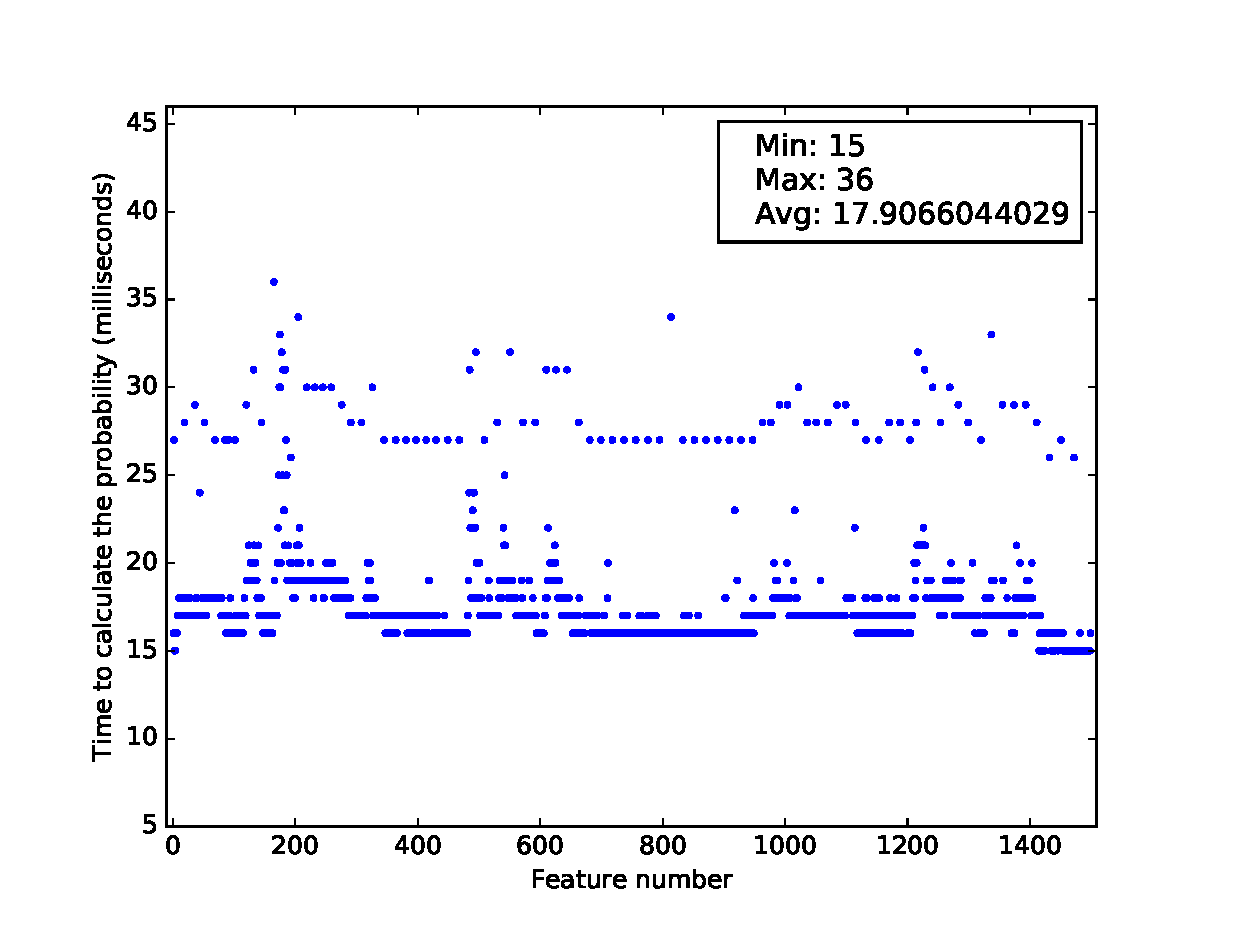
\includegraphics[width=0.8\hsize,angle=0]{plot_probs_times.eps}
	\linefigure
	\caption{Computing time analysis for a model consisting of 1500 features.}\label{fig:plot:probs:times}
\end{figure}

Figure~\ref{fig:plot:probs:times} shows the computing time required to calculate the probability of having
each feature in a product. In this case, the total time to obtain the probability for all the features is linear with respect to the total length of the analyzed term\mncomment{Que quiere decir esto? Suena raro porque yo esperaria complejidad $O(2^n)$ siendo $n$ el numero de probabilidades que salen en el termino. Pero vamos, que yo no  se mucho de complejidad!}. However, there is a small variation in the processing time for calculating the probability of each single feature. We think that his variation in mainly caused by the inherent noise of the node where the experiment is launched (e.g. disk latencies, operating
system overhead, memory paging, etc.) and, therefore, it is not related to the algorithm itself.

Since the processing time for each feature is relatively low, being around milliseconds, a single delay in
the process scheduling may have a direct impact in the overall algorithm performance. Hence, this overhead
can be considered insignificant since, in general, the time for processing each feature in the model ranges
from 15 to 28 milliseconds.

The model used in the experiments has been executed several times, providing similar results. That is, the
major part of the features require between 15 and 20 milliseconds to be processed, while there is a small
portion of them requiring a processing time between 20 and 38 milliseconds.

\begin{figure}[h]
	\centering
	\linefigure
	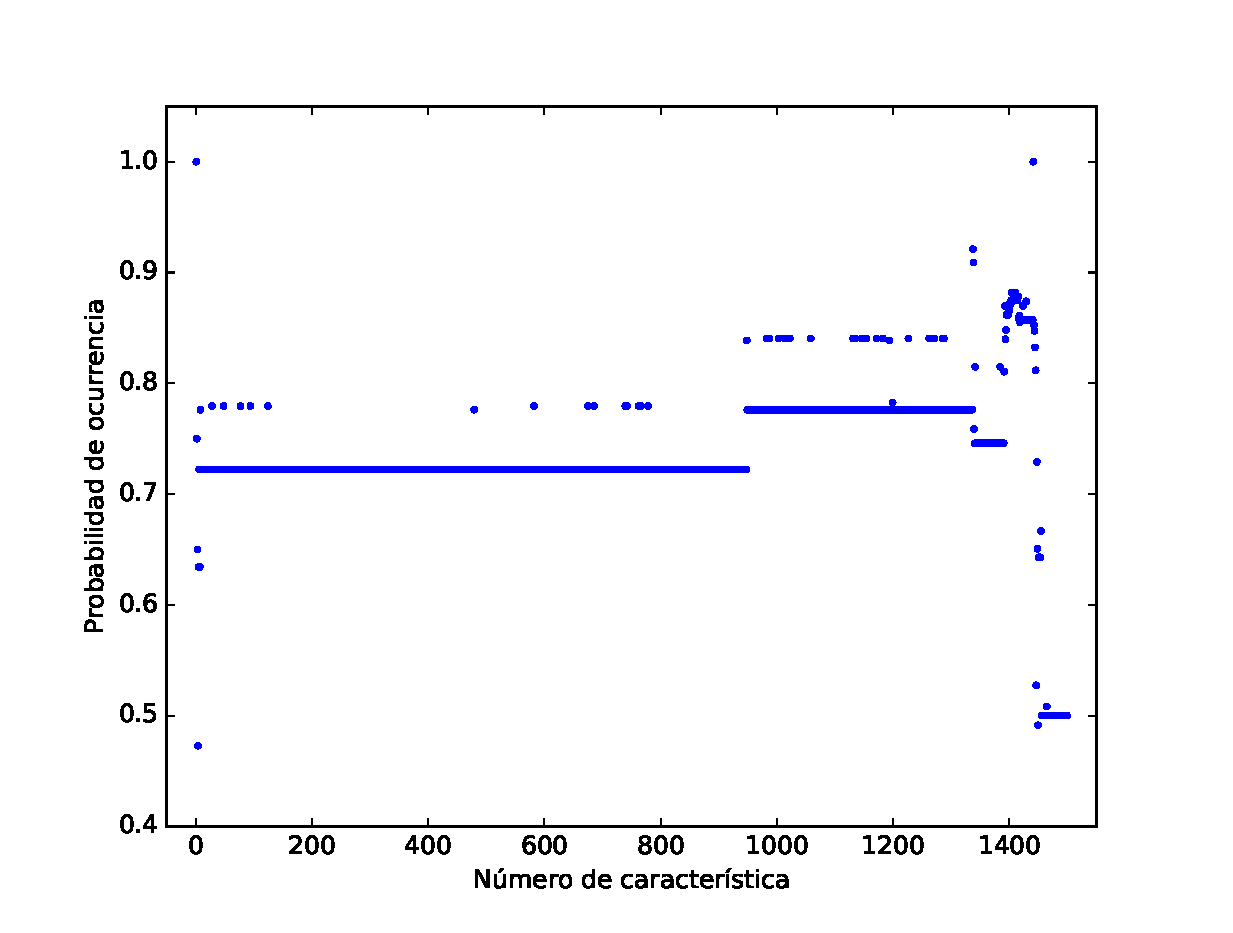
\includegraphics[width=0.8\hsize,angle=0]{plot_probs_probs.eps}
	\linefigure
	\caption{Probabilistic analysis for a 1500 features model.}\label{fig:plot:probs:probs}
\end{figure}

Figure~\ref{fig:plot:probs:probs} shows the probability of each feature in the analyzed model, where the $x$-axis
represents the feature ID and the $y$-axis represents the probability. For the sake of clarity, we provide a chart by sorting the features using its probability as sorting criteria (see Figure~\ref{fig:plot:probs:probs:sorted}).
This chart clearly shows that there exist different groups of features having a similar probability.
%
In this case, there are 450 features with, at least, a probability equal to 0.75 of being in a final product. As a conclusion,
this analysis might allow us to establish that by testing only the 28\% of the software product line components, we can ensure that 
%the features
%included in,
at least, the 75\% of the generated products, are tested.\mncomment{He reescrito un poco esta frase porque no la entendia. Please, check}

\begin{figure}[h]
	\centering
	\linefigure
	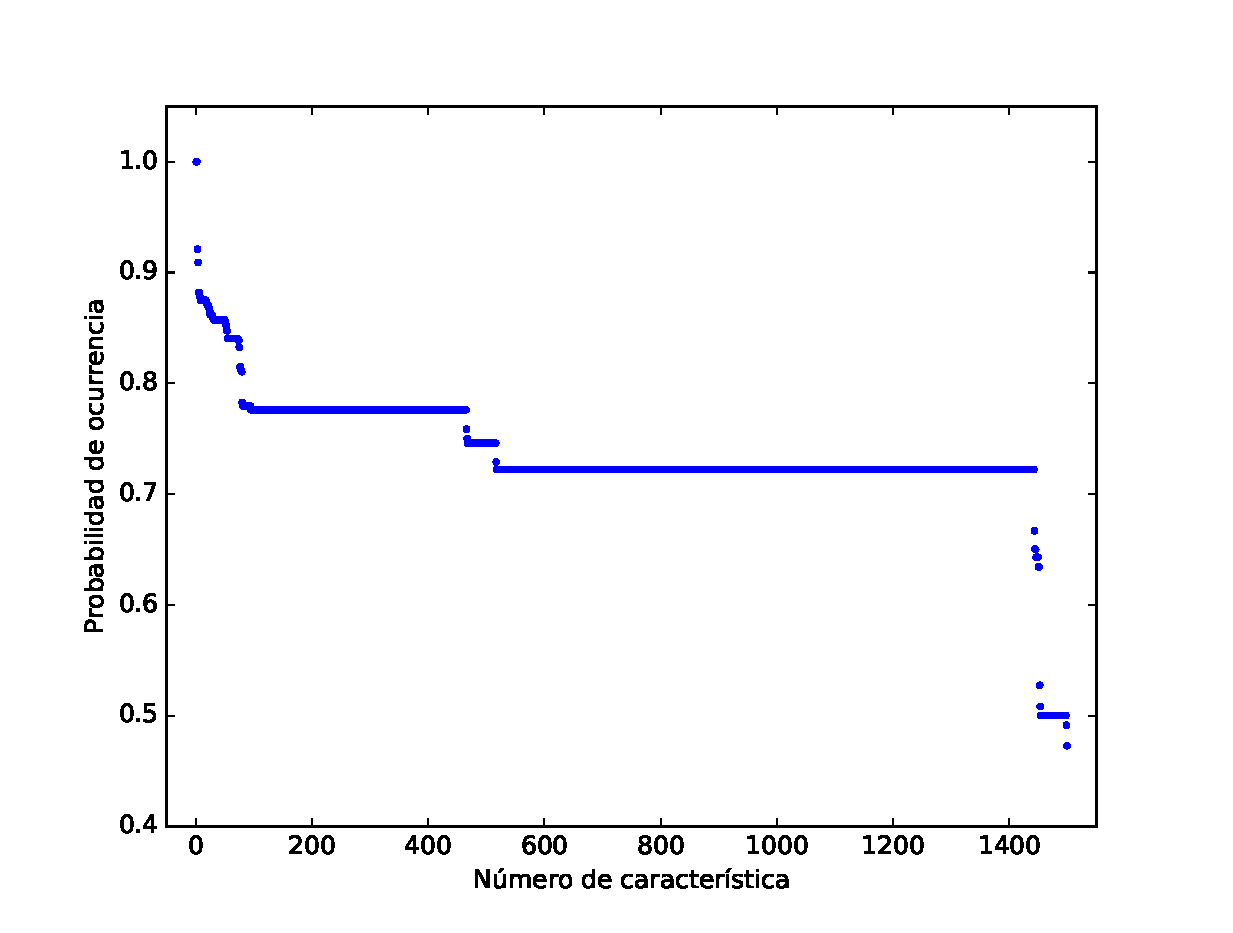
\includegraphics[width=0.8\hsize,angle=0]{plot_probs_probs_sorted.eps}
	\linefigure
	\caption{Probabilistic analysis for a 1500 features model, decreasingly sorted.}\label{fig:plot:probs:probs:sorted}
\end{figure}

%\begin{figure}[t]
%$$
%\begin{array}{ccc}
%\mathtt{Test}&\mathtt{Features}& \mathtt{Time}\\
%\#1& \feature{A},\feature{B} & 10\ units\\
%\#2& \feature{C},\feature{D} & 15\ units\\
%\#3& \feature{A},\feature{C},\feature{D} & 8\ units\\
%\#4& \feature{C},\feature{B} & 9\ units\\
%\end{array}
%$$
%\caption{Input parameter: test suite\label{fig:input:parameter}}
%\end{figure}

%We have two open issues:
%\begin{description}
%\item[Unit testing]  Let $P$ be a software product line, and $T_{unit}$ be a
%  test suite. Each test checks the correctness of a feature (i.e, %\feature{A} or \feature{B}).
%  We can compute the \emph{probability} of a feature. We test before those features with bigger probability.
%  \begin{itemize}
%  \item We can calculate the most frequent set of features in $P$ to test.
  %\item  We can provide a coverage of the test suite taking into account the percentage of appearance of each feature.
  %\end{itemize}

%\item[Integration testing] We have a test suite $T_{integration}$ where each test checks
%  the integration of a product.
%  Let us note that the integration of the product $\{\feature{A},\feature{B}\}$  can be different than
%  the integration of $\{\feature{A}, \feature{B},\feature{C}\}$.
%  \begin{itemize}
%  \item Which tests of the suite can be applied in this SPL?
 % \item What is the coverage of each test suite?
 % \end{itemize}


%\end{description}


%Next step is to associate to each integration test the time that
%it needs to be completed.
%For instance in Figure~\ref{fig:input:parameter} we represent some integration tests and the
%time that they need to be completed.



%\begin{quote}
%\emph{Let us consider an integration test suite and a probabilistic SPL $P$.
%If we only have $n$ time units, which is the \emph{best set} of tests
%to check the correctness of $P$? We say that a test is better than another
%test if its representativity (the probability to perform these features together) is higher.}
%\end{quote}

%\bprop
%        The previous problem is NP-hard\ccomen{I propose the transformation into the Subset Sum problem.}.
%\eprop

%Next we define the subset sum problem.

%\bdfn
%    Let $A = \{a_1, a_2, \ldots, a_n\}$ be a  set of natural numbers and $s$ be  a positive integer.
%    The subset sum problem checks if there is a subset $A'\subseteq A$ such that:  $$\sum_{a\in A'} = s$$
%\edfn

%In our previous problem we have a set of pairs $B=\{(p_{1},t_{1}),(p_{2},t_{2}),\ldots,(p_{n},t_{n})\}$ where
%$p_{i}$ is the probability to perform the test $i$ and $t_{i}$ is the time needed to perform this test, and
%two constants $P$ and $T$. $P$ will represent a probability value and $T$ a time value.
%We are looking for those pairs $(p_{i},t_{i}),\ldots,(p_{j},t_{j})\in B$ that
%$$
%\begin{array}{ll}
%p_{i}+\ldots +p_{j} &\geq P\\
%t_{i}+\ldots +t_{j} &\leq T\\
%\end{array}
%$$

%Let us consider that $p_{i}=t_{i}={a_i}$ and $P=T=s$.
%We can rewrite the previous problem into

%$$
%\left.
%\begin{array}{ll}
%a_{i}+\ldots +a_{j} &\geq s\\
%a_{i}+\ldots +a_{j} &\leq s\\
%\end{array}
%\right\}=
%a_{i}+\ldots +a_{j} = s\
%$$

%And we have the subset sum problem\ccomen{Please check because $p_{i}$ and $t_{i}$ can be reals while $s_{i}$ are integers}.


%\begin{enumerate}
%        \item We can create a GA to solve this problem.
%        \item We have that this problem is FPTAS~\cite{Ibarra:1975:FAA:321906.321909}.
%\end{enumerate}



%In order to obtain a set of tests that holds the previous issues, we propose
%two implementations.
%The first one is using a dynamic algorithm while the second one to use a genetic algorithm.

%\subsection{Dynamic algorithm}

% We adapted the dynamic algorithm of 0-1 Knapsack problem
%to our problem and we implemented it in python.


%We define a matrix $A$, where $A(i,j)$ contains the
%maximum value that can be attained from considering
%only the sum of the first i tests' probability that need at most j time units.


%$$
%A(i,j)=
%\left\{
%        \begin{array}{lll}
%        0 &\hspace*{3em}&\si i=0 \lor j = 0\\
%        A(i-1,j) & & \si t_i>j\\
%        \max{(A(i-1,j),p_{i}+A(i-1,j-t_i))} &&\si t_i \leq j
%        \end{array}
%\right.
%$$

%In our case, we will say that $A(n,T)$ is the solution if the sum of the  percentages
%of all elements involved in this solution is bigger than or equal to $P$. Otherwise we do not have a solution.


%For instance, in Table~\ref{figure:input:parameters} there are presented a set of 24
%different tests with their time consuming and its probability.
%For instance the first element, t1,9,150, means the test t1 needs 9 time units to be completed
%and the value associated with this test is 150\footnote{We could put here a measure, the probability or anything}.

%\begin{table}
%\centering

%\selectfont
%{\tt
%\begin{tabular}{|l|l|l|}
%\hline
%\#1,9,150 &
%\#2,13,35&
%\#3,153,200\\
%\#4,50,160&
%\#5,15,60&
%\#6,68,45\\
%\#7,27,60&
%\#8,39,40&
%\#9,23,30\\
%\#10,52,10&
%\#11,11,70&
%\#12,32,30\\
%\#13,24,15&
%\#14,48,10&
%\#15,73,40\\
%\#16,42,70&
%\#17,43,75&
%\#18,22,80\\
%\#19,7,20&
%\#20,18,12&
%\#21,4,50\\
%\#22,30,10&
%\#23,90,1&
%\#24,200,150\\
%\hline
%\end{tabular}}
%\caption{Input parameter (test,time,value) for the test selection algorithm.\label{figure:input:parameters}}
%\end{table}

% \begin{figure}[t]
% \centering
% includegraphics[scale=1]{GA_Flowchart_4}
% \caption{Scheme of GA.\label{scheme:genetic:algorithm}}
% \end{figure}





% After executing the dynamic algorithm, with the following input parameters a)
% the data presented in Table~\ref{figure:input:parameters} and T (the maximum time value) equals to 500,
% we obtain that {\tt \#1, \#2, \#3, \#4, \#5,
% \#7, \#8, \#9, \#11, \#12, \#16, \#17,
% \#18, \#19} and {\tt \#21}       conforms the final solution, and P =  1130.


% \subsection{Genetic Algorithm}

% Next we perform a genetic algorithm to discover a better solution.
% The GA structure is in Figure~\ref{scheme:genetic:algorithm}.
% With this algorithm we obtain values bigger than 1130.






% \subsubsection{Representation}
% We represent the possible solutions (those tests that hold the conditions) as follows:
% \begin{itemize}
%         \item Genotype: Given $n$ tests, we represent a solution with a binary (1/0) string
% of length $n$ where the position i determines whether the ith-test is included or not.
% The genotype space is complete, that is, any valid solution can be mapped in this array.
%         \item Phenotype: There are only some genotypes that are \emph{correct}. These are
% those that taking the $n'$, with $n'\leq n$ first $1$ bits from left to right of a genotype, we have that the sum of
% the time values associated with these tests is lower than or equal to T,
% and that the representativity of these tests is $\geq P$.
% \end{itemize}


% \subsubsection{Initial Population}
% We execute the algorithm with the parameters presented in Figure~\ref{fig:parameters:initial:population} in order to show
% how many initial population do we need.
% There is an interesting effect that this experiment reveals.
% The first and second graphs indicate that for populations smaller than 50 the chance for premature convergence seems to be rather high.
% Therefore we will consider that a good candidate for initial population is 500.

% \begin{figure}[t]
% \centering

% \begin{minipage}{0.45\hsize}\centering
%         \textbf{x}=10

% \includegraphics[scale=0.3]{graphs_basea/basea_diff_raw}
% \end{minipage}
% \begin{minipage}{0.4\hsize}\centering

%         \textbf{x}=50
% \includegraphics[scale=0.3]{graphs_baseb/baseb_diff_raw}

% \end{minipage}


% \begin{minipage}{0.45\hsize}\centering
%         \textbf{x}=200

% \includegraphics[scale=0.3]{graphs_based/based_diff_raw}
% \end{minipage}
% \begin{minipage}{0.4\hsize}\centering

%         \textbf{x}=500
% \includegraphics[scale=0.3]{graphs_basec/basec_diff_raw}

% \end{minipage}

% {\centering
% %\fontsize{7}{9}
% %\selectfont

% \begin{tabular}{|l|l|}
% \hline
% Representation  &Binary strings of length n\\
% Recombination   &One point crossover\\
% Recombination probability &     80\\
% Mutation        & Swap Mutator \\
% Mutation probability    & 2\% \\
% Parent selection        & Roulette\\
% Survivor selection      & Generational\\
% Population size         & \textbf{x} \\
% Termination condition   & Terminate the evolution based on the fitness stats\\
% Generations     & 100 \\
% \hline
% \end{tabular}}

% \caption{Comparing initial population\label{fig:parameters:initial:population}.}
% \end{figure}



% \subsubsection{Recombination probability}
% Next we study the effect of changing the recombination probability.
% In Figure~\ref{fig:parameters:recombination} we show the max fitness, average fitness and
% minimum fitness of the population, in each generation, using the probability values 0.1, 0.4, 0.8 and 1 for recombination.
% We will use 0.8 in the rest of experiments because a) we obtain the maximum fitness, and b) the difference between maximum and minimum is low.

% Let us also note that adding more values of recombination probability (i.e, 100\%), that is also presented in
%  Figure~\ref{fig:parameters:recombination} does not imply to have better fitness solutions. So, this value should be high
% but not 100\%.

% \begin{figure}[t]

% \centering

% \begin{minipage}{0.5\hsize}\centering
%         \textbf{x}=0.1

% \includegraphics[scale=0.3]{graphs_basee/basee_maxmin_fitness}
% \end{minipage}
% \begin{minipage}{0.4\hsize}\centering

%         \textbf{x}=0.4
% \includegraphics[scale=0.3]{graphs_basef/basef_maxmin_fitness}

% \end{minipage}


% \begin{minipage}{0.50\hsize}\centering
%         \textbf{x}=0.8

% \includegraphics[scale=0.3]{graphs_baseg/baseg_maxmin_fitness}
% \end{minipage}
% \begin{minipage}{0.4\hsize}\centering

%         \textbf{x}=1
% \includegraphics[scale=0.3]{graphs_baseh/baseh_maxmin_fitness}

% \end{minipage}


% {\centering
% %\fontsize{7}{9}
% %\selectfont

% \begin{tabular}{|l|l|}
% \hline
% Representation  &Binary strings of length n\\
% Recombination   &One point crossover\\
% Recombination probability &     \textbf{x}\\
% Mutation        & Swap Mutator \\
% Mutation probability    & 2\% \\
% Parent selection        & Roulette\\
% Survivor selection      & Generational\\
% Population size         & 500 \\
% Termination condition   & Terminate the evolution based on the fitness stats\\
% Generations     & 100 \\
% \hline
% \end{tabular}}

% \caption{Comparing recombination probability\label{fig:parameters:recombination}.}
% \end{figure}

% \subsubsection{Mutation operator}

% We define two mutation operators in the chromosomes. The first one: swap means to change
% the element i with the element j. The second one: Integer range, means that we change a bit
% randomly.

% In our algorithm we are able to use both mutators operators.
% In Figure~\ref{fig:parameters:mutation:operator} the effects of executing swap, integer range or both
% are presented.

% We can observe that only swap let the fitness score to be regular with respect to the number of generations.
% When we change randomly a bit in the chromosomes then the fitness score cannot be predictable.

% \begin{figure}[t]

% \centering

% \begin{minipage}{0.5\hsize}\centering
%         \textbf{x}=Swap

% \includegraphics[scale=0.3]{graphs_basei/basei_maxmin_fitness}
% \end{minipage}
% \begin{minipage}{0.45\hsize}\centering

%         \textbf{x}=Swap and Integer Range

% \includegraphics[scale=0.3]{graphs_basej/basej_maxmin_fitness}

% \end{minipage}

% \begin{minipage}{0.5\hsize}\centering
%         \textbf{x}=Integer Range

% \includegraphics[scale=0.3]{graphs_basek/basek_maxmin_fitness}
% \end{minipage}
% %\begin{minipage}{0.45\hsize}\centering

% {\centering

% %\fontsize{7}{9}
% %\selectfont
% \begin{tabular}{|l|l|}
% \hline
% Representation  &Binary strings of length n\\
% Recombination   &One point crossover\\
% Recombination probability &     0.8\\
% Mutation        & \textbf{x} \\
% Mutation probability    & 2\% \\
% Parent selection        & Roulette\\
% Survivor selection      & Generational\\
% Population size         & 500 \\
% Termination condition   & Terminate the evolution based on the fitness stats\\
% Generations     & 100 \\
% \hline
% \end{tabular}}
% %\end{minipage}

% \caption{Comparing Mutation Operators\label{fig:parameters:mutation:operator}.}
% \end{figure}

% \subsubsection{Parent Selection}

% Finally we compare the parent selection methodology used in our algorithm.
% We implement three kind of selections: Rank, Roulette and Tournament.
% In our experiments we decided to use Roulette because it is always increasing,
% and it seems that we can continue improving the valuation of the set of tests over time.
% Moreover the others seem to be saturated.
% \begin{figure}[t]

% \centering

% \begin{minipage}{0.5\hsize}\centering
%         \textbf{x}=Rank

% \includegraphics[scale=0.3]{graphs_baser/baser_maxmin_fitness}
% \end{minipage}
% \begin{minipage}{0.4\hsize}\centering

%         \textbf{x}=Roulette
% \includegraphics[scale=0.3]{graphs_bases/bases_maxmin_fitness}

% \end{minipage}

% \begin{minipage}{0.50\hsize}\centering
%         \textbf{x}=Tournament

% \includegraphics[scale=0.3]{graphs_baset/baset_maxmin_fitness}
% \end{minipage}

% %\begin{minipage}{0.45\hsize}\centering


% {\centering
% %\fontsize{7}{9}
% %\selectfont
% \begin{tabular}{|l|l|}
% \hline
% Representation  &Binary strings of length n\\
% Recombination   &One point crossover\\
% Recombination probability &     0.8\\
% Mutation        & Swap \\
% Mutation probability    & 2\% \\
% Parent selection        & \textbf{x}\\
% Survivor selection      & Generational\\
% Population size         & 500 \\
% Termination condition   & Terminate the evolution based on the fitness stats\\
% Generations     & 100 \\
% \hline
% \end{tabular}}
% %\end{minipage}

% \caption{Comparing parent selection\label{fig:parameters:parent:selection}.}
% \end{figure}

%%% Local Variables:
%%% mode: latex
%%% TeX-master: "main"
%%% End:

